%%
% 第五章 双图架构改进与效果分析
% 在原架构基础上引入残基级 GVP 通路
% 单折观察：AUC 微幅提升 + AUPR 回落 → 架构工程可行性，不作性能超越结论
%%

\chapter{双图架构改进与效果分析}
\label{cha:dualgraph}

本章以第四章原架构基线模型（M0）为对照，提出并实现双图架构改进模型（M1），在原子级结构通道之外并行引入残基级几何向量感知通路。本章依次阐述原架构在方向信息编码上的局限、双图架构的设计动机与原理、残基级几何向量感知模块的具体实现，以及在第三章统一数据集与第四章相同训练配置下的训练与测试结果；最后对所得观察给出严格限定于单随机切分评估范围内的讨论与方法学启示。

\section{原架构对方向信息的局限性}
\label{sec:ch5-limitation}

原架构模型 M0 的结构通道采用 E($n$)-等变图神经网络（E($n$)-equivariant graph neural network，EGNN）\cite{EGNN2021} 对对接复合物的原子图进行消息传递。EGNN 在坐标层面对旋转--平移--反射等变，而其用于下游交叉注意力的标量节点特征则对刚体变换不变；这一不变性使模型对分子在空间中的姿态变化鲁棒，但代价是\textbf{送入下游交叉注意力的标量表示难以显式保留方向信息}：对于活性位点中相距 $2.8~\mathrm{\AA}$ 的两个氧原子，无论它们位于底物上方还是下方，EGNN 输出到交叉注意力的标量特征几乎不可区分，方向信息在池化之前已被实质性弱化。

这一局限对 P450 家族的特异性预测尤为不利。P450 的催化中心为血红素铁（heme-Fe），底物需通过狭长的底物通道进入活性口袋并以特定朝向接近 Fe 以保证羟化反应的区域选择性；P450 催化机理研究表明，底物 C--H 键相对血红素铁活性氧的朝向是决定羟化反应区域选择性的核心几何因素\cite{Guengerich2008}。原子级 EGNN 在 $10~\mathrm{\AA}$ 口袋内虽然刻画了距离关系，但其标量特征通道无法表达 Fe--底物--口袋残基之间的方向与朝向信息。原架构 M0 的整体结构示意见图~\ref{fig:ch5-baseline}：序列、结构与分子三通道并行，以双向交叉注意力将酶残基与底物原子相互参考，最终拼接七个 128 维向量送入预测头。由此产生一个自然的改进方向：在不破坏原子级 EGNN 通路的前提下，引入一条具备方向感知能力的几何编码通路，补足结构通道的表征维度。

\begin{figure}[!htbp]
  \centering
  \makebox[\textwidth][c]{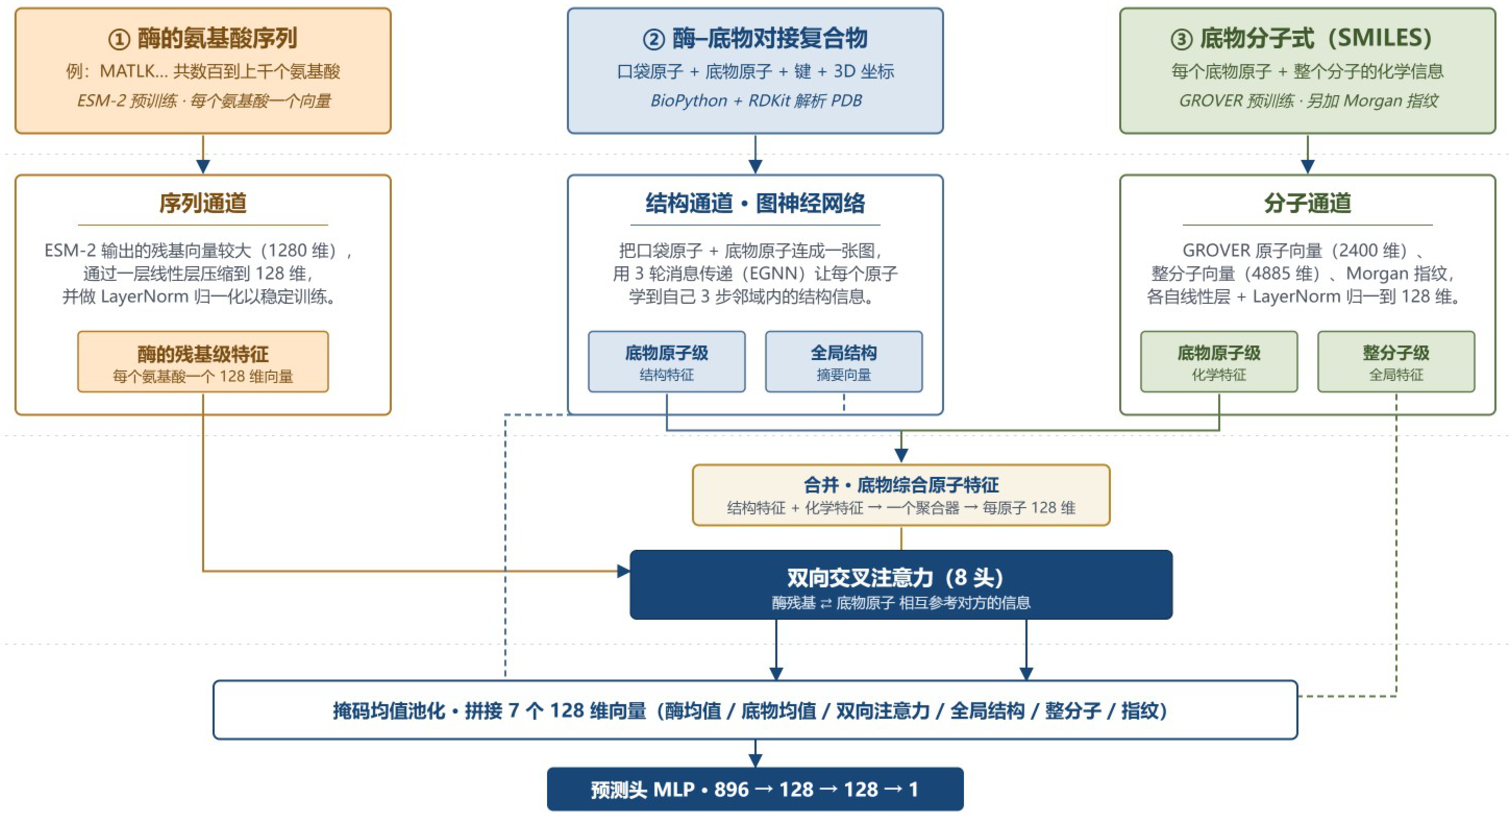
\includegraphics[width=1.25\textwidth]{./image/原始架构.pdf}}
  \caption{原架构 M0 总体示意：序列、结构与分子三通道并行编码，经双向交叉注意力使酶残基与底物原子互相参考，最终拼接 7 个 128 维向量送入预测头 MLP 输出二分类 logits}
  \label{fig:ch5-baseline}
\end{figure}

\section{双图架构设计动机与原理}
\label{sec:ch5-design}

\subsection{几何向量感知器（Geometric Vector Perceptron，GVP）}
\label{subsec:ch5-gvp}

GVP\cite{GVP2021} 是一类 SE(3)-等变（SE(3)-equivariant）层，区别于 SE(3)-不变层的根本特征在于：GVP 同时接受并输出两类表示——标量通道按常规神经网络方式变换，向量通道在空间旋转下"跟着转"。对整个口袋做整体旋转时，GVP 的标量输出保持不变，而向量输出以整体旋转矩阵作用后的新坐标给出。这一特性使 GVP 天然适合表达残基骨架朝向、侧链指向等方向依赖信息，而又不丢失原子级 EGNN 所依赖的距离关系。

基于上述考虑，本研究提出\textbf{双图架构}：在原架构保留原子级 EGNN 通路完全不变的基础上，新增一条残基级 GVP 通路与之并行运行。每个口袋残基被打包为一个节点，含"标量部分 + 向量部分"两组特征。\textbf{标量部分}用骨架主链二面角 $\varphi$、$\psi$、$\omega$ 的 $\sin$、$\cos$ 编码共 $6$ 维表达骨架的局部折叠构象；\textbf{向量部分}用 $\mathrm{C}\alpha \to \mathrm{N}$、$\mathrm{C}\alpha \to \mathrm{C}$、$\mathrm{C}\alpha \to \mathrm{C}\beta$ 三个三维方向向量共 $3 \times 3$ 维表达骨架朝向与侧链指向。残基节点之间的连边取每个残基空间最近邻 30 个残基，边特征含 $\mathrm{C}\alpha$--$\mathrm{C}\alpha$ 距离的径向基函数展开与 $\mathrm{C}\alpha$--$\mathrm{C}\alpha$ 方向向量。整个口袋旋转时 GVP 的标量输出不变、向量输出跟随旋转，几何关系被完整保留而不会被 SE(3)-不变所抛弃。

\subsection{双出口融合设计}
\label{subsec:ch5-fusion}

GVP 通路的输出（每残基 256 维，记为 $\mathbf{h}_{\mathrm{res}}$）通过两条独立路径注入主网络（见图~\ref{fig:ch5-arch}）。\emph{出口一（深融合）}将 $\mathbf{h}_{\mathrm{res}}$ 经线性层压至 128 维后按残基映射回注到序列通道的残基级特征之上，以更新双向交叉注意力\cite{Transformer2017} 的查询端；\emph{出口二（浅旁路）}将 $\mathbf{h}_{\mathrm{res}}$ 做残基均值池化压至 128 维，直接拼接入掩码池化后的综合向量。原架构在掩码池化后拼接的综合向量含 7 个 128 维分量（共 896 维），引入浅旁路后扩为 8 个分量（共 1024 维），随后送入多层感知机预测头输出二分类 logits。

\begin{figure}[!htbp]
  \centering
  \makebox[\textwidth][c]{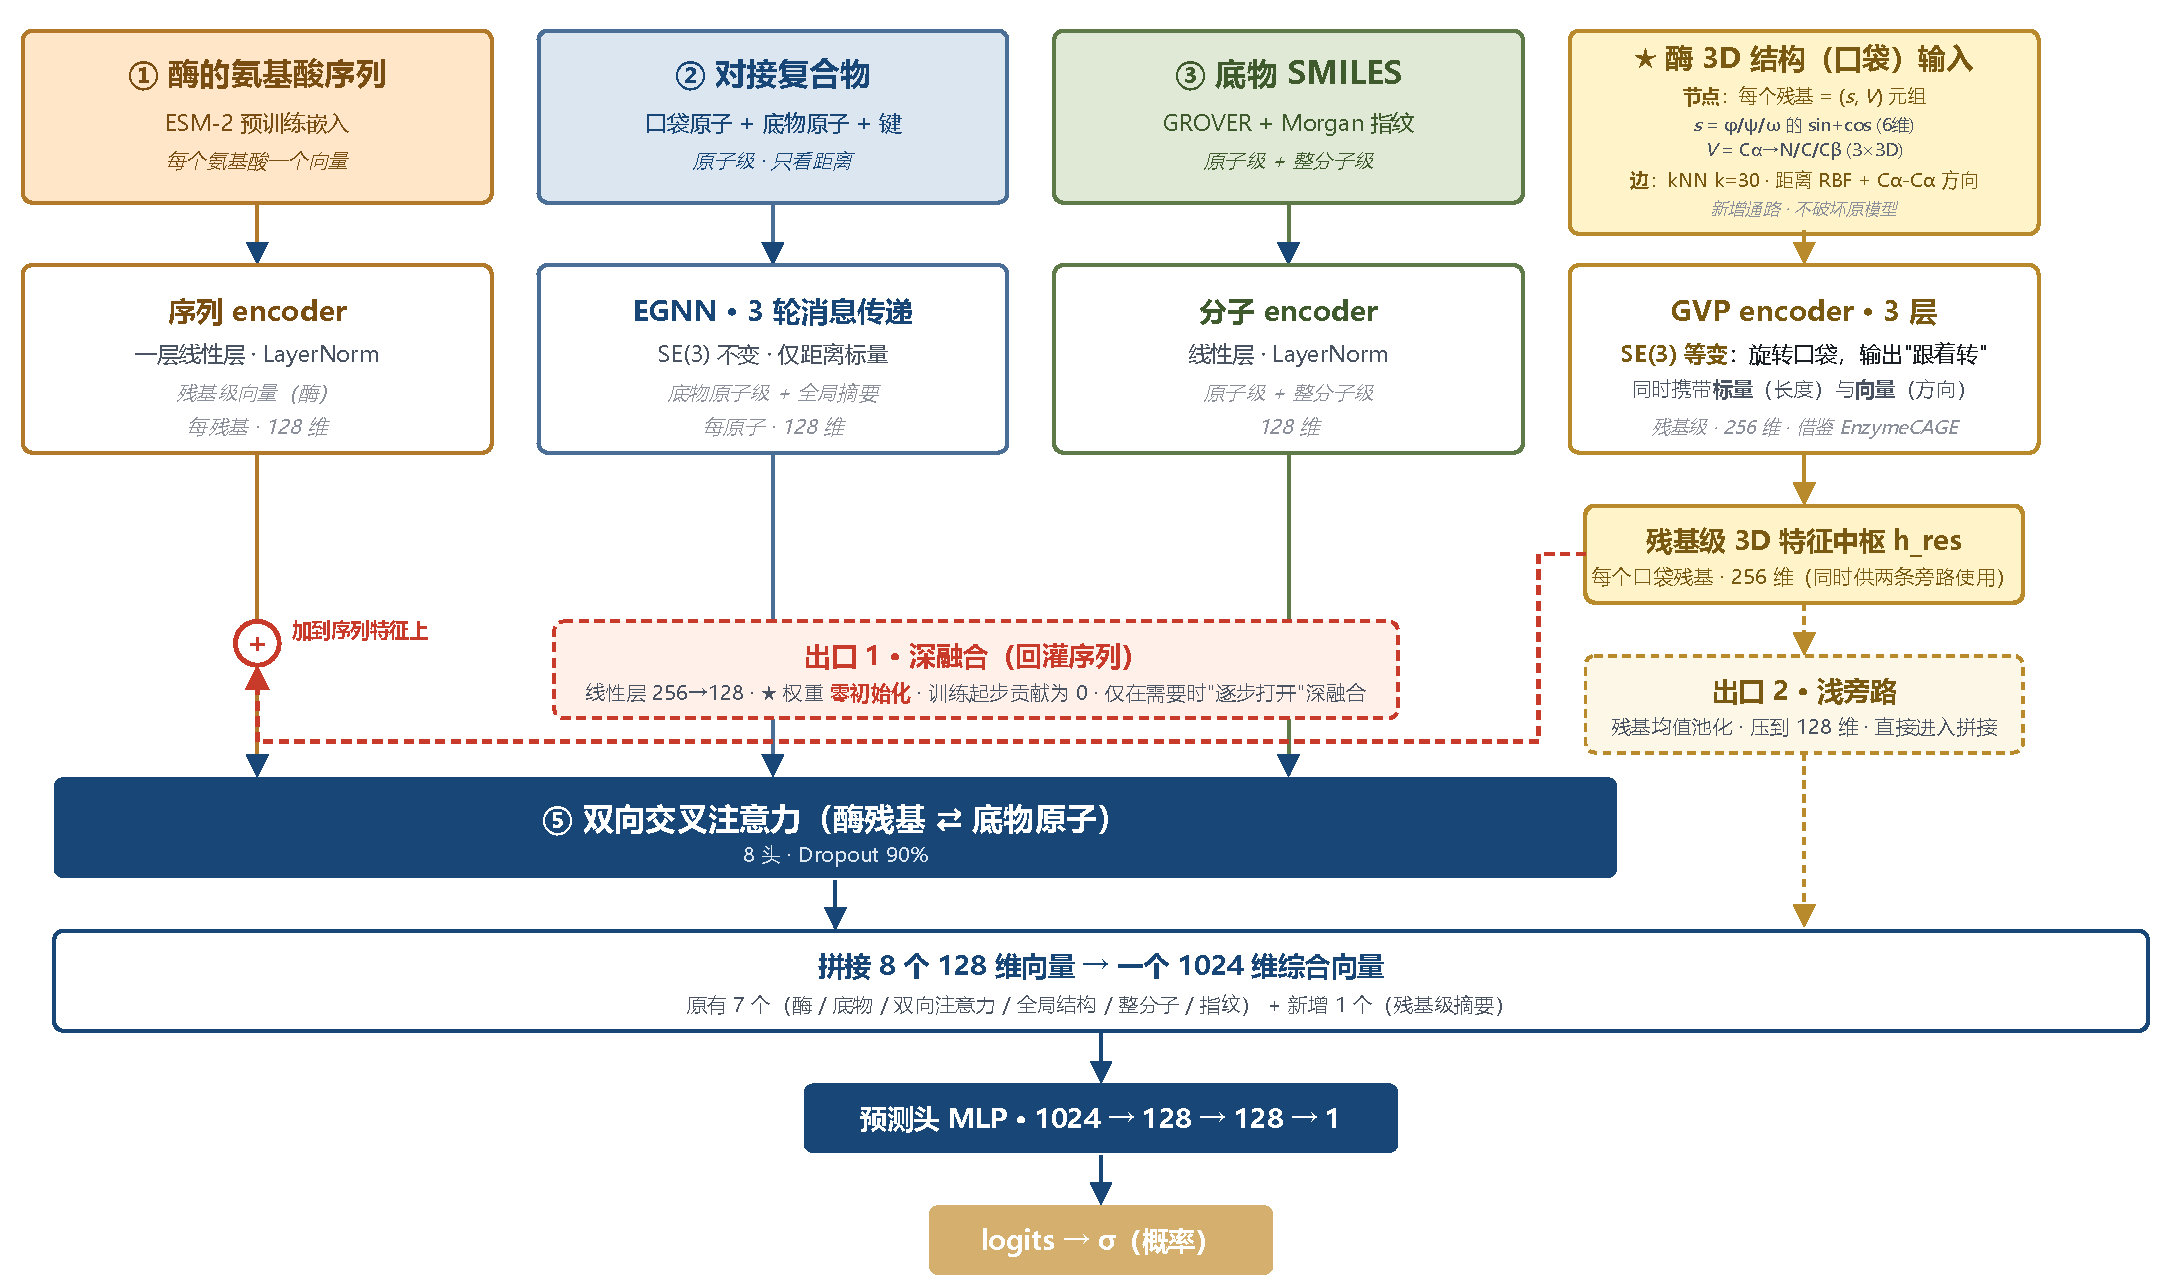
\includegraphics[width=1.25\textwidth]{./image/双图架构.pdf}}
  \caption{双图架构示意图：在原架构三通道基础上并行引入残基级 GVP 通路（右侧新增分支），输出经"出口一深融合"回灌序列通道、"出口二浅旁路"接入末端综合向量；零初始化与延迟解冻保证训练第 0 步与 M0 严格等价}
  \label{fig:ch5-arch}
\end{figure}

\section{残基级几何向量感知模块的实现}
\label{sec:ch5-implementation}

\subsection{GVP 编码器}
\label{subsec:ch5-encoder}

GVP 编码器由 3 层 GVP 构成，每层交替执行标量更新与向量更新，层间残差连接。实现上借鉴了公开的 GVP 参考实现\cite{GVP2021} 以及在酶--底物特异性任务上应用残基级 GVP 的 EnzymeCAGE 工程实现\cite{EnzymeCAGE2026}，并针对本研究的口袋数据规模（每口袋约 $30$--$100$ 个残基）调整了近邻半径与批处理策略。

\subsection{严格的基线等价性验证}
\label{subsec:ch5-equiv}

为避免双图架构在训练起步阶段对原架构 M0 的已有权重产生扰动，本研究对融合点做了\textbf{权重零初始化}：出口一深融合的线性层末层权重初始化为 $0$、出口二浅旁路在预测头中对应的新增 $128$ 维分量权重同样零初始化。在此设置下，模型第 0 步的前向输出严格等于原架构 M0，数值上最大绝对偏差为 $4 \times 10^{-8}$。这一验证确保了双图架构的效果差异只能来自训练过程中被梯度激活的 GVP 通路，而非初始化扰动。

\subsection{延迟解冻策略}
\label{subsec:ch5-unfreeze}

与零初始化配合，本研究采用延迟解冻：第 0 步时 GVP 分支所有参数梯度为 $0$、不参与权重更新；第 1 步起 GVP 分支被解冻并开始被梯度驱动。该设计使得训练起步与原架构完全一致、随即逐步激活新分支。由于第 0 步 GVP 分支存在参数但不参与反向传播，在分布式数据并行（Distributed Data Parallel，DDP）训练下需将 \texttt{find\_unused\_parameters} 设置为 \texttt{True} 以避免 PyTorch 的严格同步检查在首步报错；该选项引入约 5\%--10\% 的同步开销，但为延迟解冻设计所必需。

\subsection{规模与训练开销}
\label{subsec:ch5-scale}

双图架构相对原架构引入约 45\% 的新参数量（$1.85~\mathrm{M} \to 2.68~\mathrm{M}$），主要来自 GVP 编码器三层与出口融合线性层；每 epoch 训练时间由原架构的约 $55$ 秒增加至约 $60$ 秒，端到端训练成本增幅可控。

\section{双图架构训练与测试结果}
\label{sec:ch5-results}

双图架构模型 M1 的训练配置与第四章 \ref{sec:ch4-config} 节一致：4 块 RTX 5090 上 DDP 并行，单卡批大小 88、有效全局批大小 352，AdamW\cite{AdamW2019} 优化器，200 epoch 最大训练轮次，验证集 AUPR 为监控指标的早停机制。唯一变化在于 DDP 配置启用 \texttt{find\_unused\_parameters}。训练在第 57 个 epoch 早停，总耗时约 $56.8$ 分钟；验证集最佳 checkpoint 出现在第 $41$ 轮，对应 Val AUC $= 0.9262$。

在与原架构 M0 完全相同的随机切分第一折测试集（10{,}999 条样本、984 正 / 10{,}015 负）上评估 M1 的最佳 checkpoint，得到 \textbf{Test AUC $= 0.9310$、Test AUPR $= 0.6474$}。与原架构 M0（ep43，Test AUC $= 0.9302$、Test AUPR $= 0.6749$）的对比结果汇总于表~\ref{tab:ch5-results}。AUC 指标维度上，双图架构相对原架构观察到 $\Delta = +0.0008$ 的\textbf{微幅提升}；AUPR 指标维度上，双图架构相对原架构观察到 $\Delta = -0.0275$ 的\textbf{回落}。两项指标并列、对称报告，如实反映本研究的单折观察结果。

\begin{table}[htbp]
  \centering
  \caption{双模型在随机切分第一折测试集上的完整结果对比}
  \label{tab:ch5-results}
  \begin{tabular}{llcccc}
    \toprule
    模型 & 最佳 ckpt & Val AUC & Test AUC & Test AUPR & 参数量 \\
    \midrule
    原架构 M0      & ep43 & 0.9250 & 0.9302 & 0.6749 & 1.85 M \\
    双图架构 M1    & ep41 & 0.9262 & \textbf{0.9310} & 0.6474 & 2.68 M \\
    \midrule
    $\Delta$（M1 $-$ M0）  & --- & $+0.0012$ & $\bm{+0.0008}$ & $-0.0275$ & $+45\%$ \\
    \bottomrule
  \end{tabular}
\end{table}

\begin{figure}[!htbp]
  \centering
  \makebox[\textwidth][c]{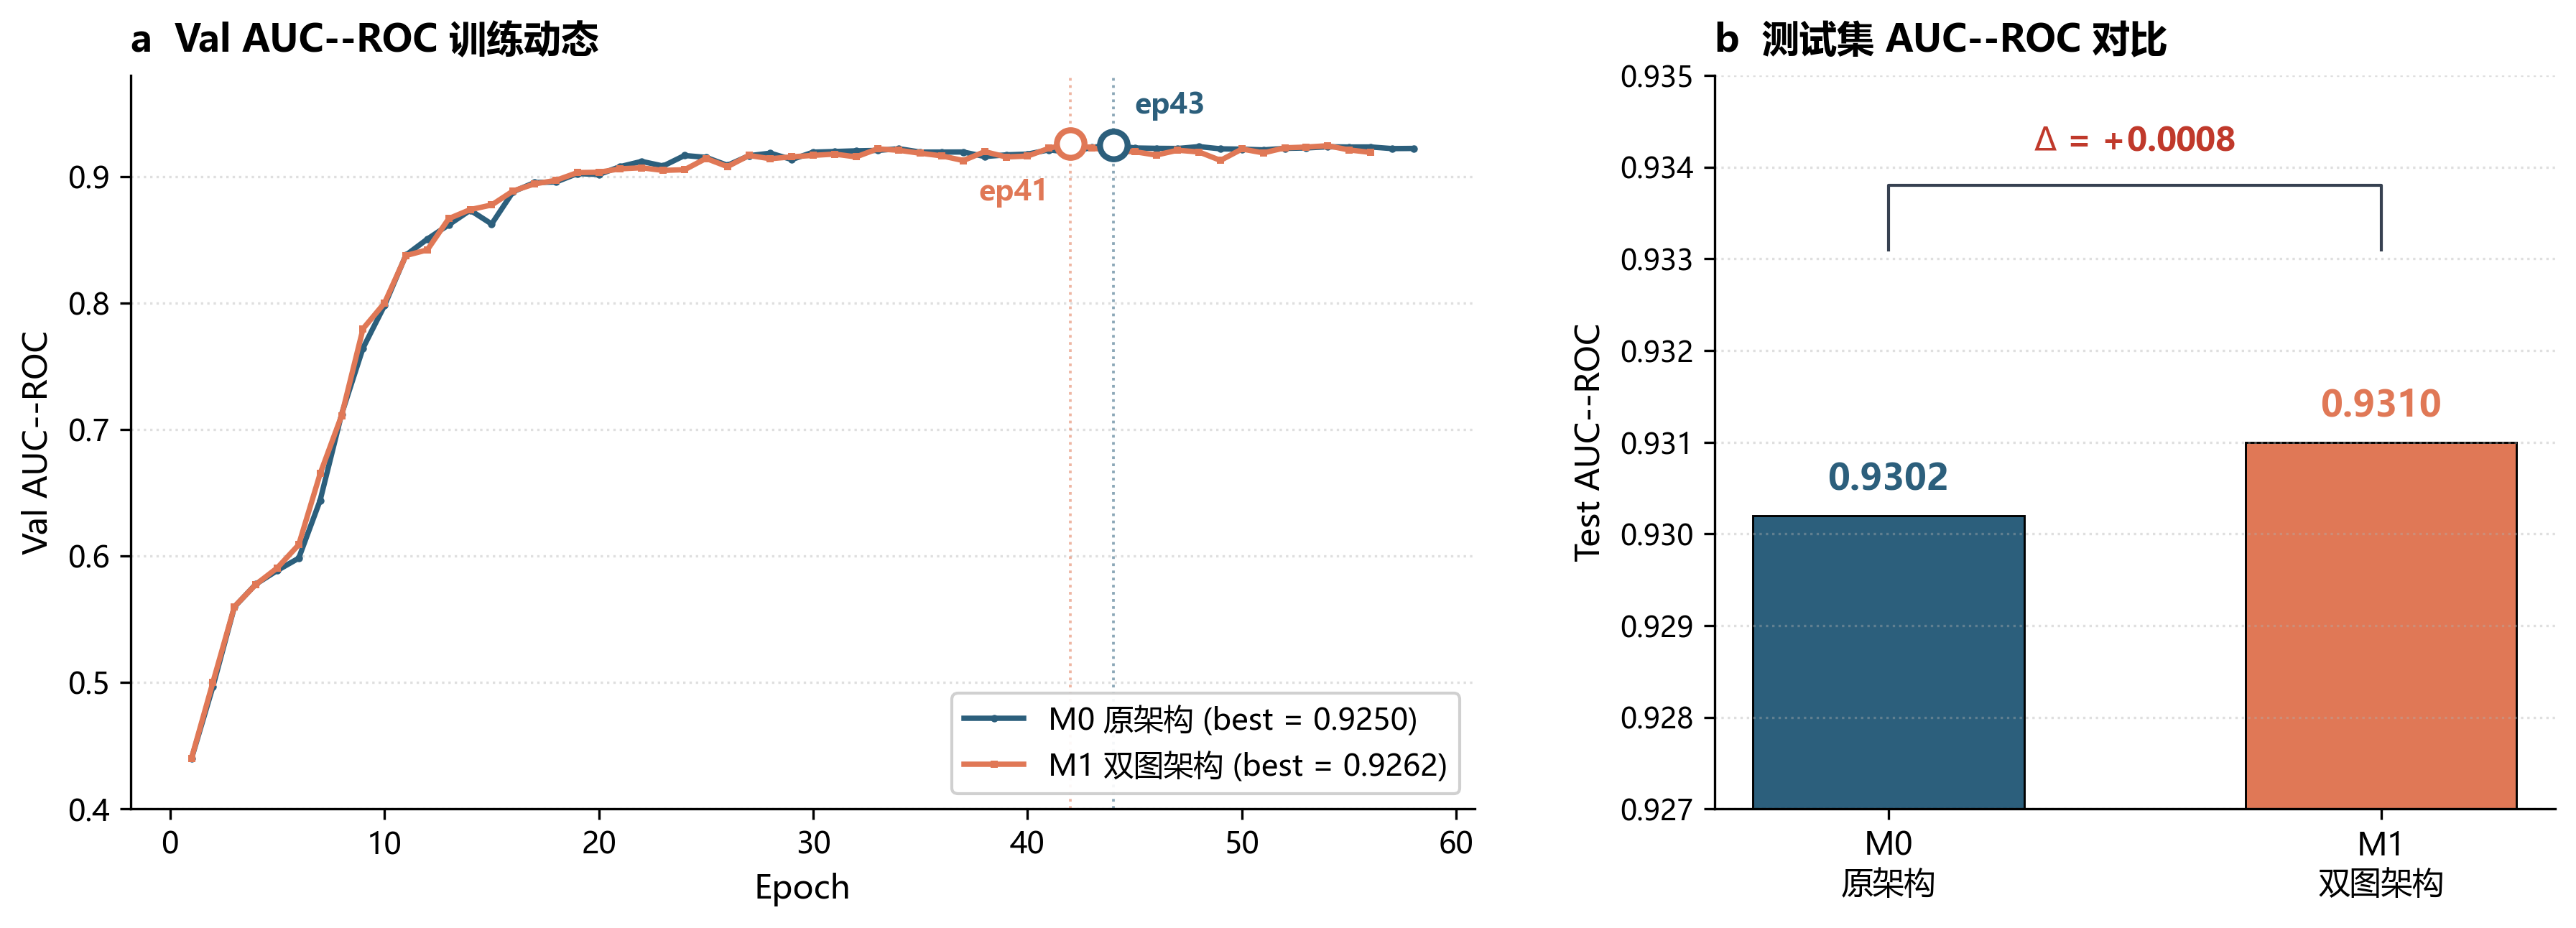
\includegraphics[width=1.15\textwidth]{./image/M0_M1对比.png}}
  \caption{原架构 M0 与双图架构 M1 对比：(a) Val AUC--ROC 训练曲线，M0 best ep43 = 0.9250，M1 best ep41 = 0.9262；(b) 测试集 AUC--ROC，M0 = 0.9302，M1 = 0.9310，$\Delta = +0.0008$}
  \label{fig:ch5-results}
\end{figure}

\section{结果讨论与方法学启示}
\label{sec:ch5-discussion}

\subsection{对单折观察的诚实解读}

上节表~\ref{tab:ch5-results} 给出的观察需要严格限定其有效范围。\textbf{AUC 微幅提升的方向}与第 \ref{sec:ch5-design} 节所述"对方向敏感的 P450 催化需要方向感知表征"物理假设方向一致，可作为双图架构\emph{架构工程层面}的初步可行性探索报告。然而，$+0.0008$ 的提升幅度处于单折评估的噪声边缘，加之训练时间（$56.8$ 分钟）与测试条件的唯一性，不足以支撑"双图架构在性能上优于原架构"的定性结论。\textbf{AUPR 的回落}同样需要诚实面对：$-0.0275$ 的下降在极不平衡数据（正负比约 $1:10$）上反映出模型对稀有正样本打分分布的扰动，其成因可能包括：未经充分超参调优情况下残基级通路导致的轻度过拟合、GVP 分支引入额外参数（$+45\%$）后在少数类上的优化困难、或单折评估本身的方差。本研究将此视为空间分辨率与优化难度之间的 trade-off 信号，不予强行淡化或选择性引用。

综合上述两点观察，本研究将双图架构定位为\textbf{对方向信息感知设计的初步可行性探索}，而非性能超越或稳健性结论。真正的稳健性判定需建立在多随机种子 $\times$ 多折交叉验证 $\times$ 充分超参调优 $\times$ 显著性检验的基础上，这些工作因单折的时间与资源限制未在本论文中完成，作为主要局限在第六章标注。

\subsection{对未来 P450 几何感知模型设计的启示}

上述受控单次观察仍对未来方法学设计提供了若干可操作的启示。第一，\textbf{方向感知通路作为距离感知通路的补充}具有进一步探索的价值：GVP 类模块在 P450 类几何敏感酶家族上虽然在本单折评估中未展现稳健的性能提升，但 AUC 方向与物理直觉一致，提示该方向值得以多折稳健评估为前提继续试验。第二，\textbf{标量--向量联合建模的工程可行性}已在本研究被验证：零初始化与延迟解冻的组合设计使得新分支可以在不破坏已有基线能力的前提下被逐步激活，该模式可推广到其他"在已训练好架构上加通路"的改进场景。第三，\textbf{极不平衡分类任务上的指标选择}不可仅依赖单一 AUC：本研究观察到的 AUC 提升与 AUPR 回落反向变化清楚说明，在正负比 $1:10$ 量级的任务上若仅报告 AUC 将遗漏对稀有正样本真实表现的关键信息；AUC 与 AUPR 并列评估应成为此类任务的默认做法\cite{Saito2015}。

本章的最终定位是：在第四章数据集层面与评估协议层面已确立的核心贡献之外，以架构工程角度补充一条带有方向感知能力的技术路线；所报告的数值观察与讨论均限定在单一随机折评估范围内，作为后续稳健性验证的起点而非终点。
